%% Customizacoes do abnTeX2 (http://abnTeX2.googlecode.com) para o IFRS Campus Osorio v1.1
%% Por Bruno Fernandes (bruno.fernandes@osorio.ifrs.edu.br)
%% O modelo mais atualizado está disponível em bit.ly/ADSLaTeX
%%
%% abtex2-modelo-trabalho-academico.tex, v-1.9.6 laurocesar
%% Copyright 2012-2016 by abnTeX2 group at http://www.abntex.net.br/ 
%%
%% This work may be distributed and/or modified under the
%% conditions of the LaTeX Project Public License, either version 1.3
%% of this license or (at your option) any later version.
%% The latest version of this license is in
%%   http://www.latex-project.org/lppl.txt
%% and version 1.3 or later is part of all distributions of LaTeX
%% version 2005/12/01 or later.
%%
%% This work has the LPPL maintenance status `maintained'.
%% 
%% The Current Maintainer of this work is the abnTeX2 team, led
%% by Lauro César Araujo. Further information are available on 
%% http://www.abntex.net.br/
%%
%% This work consists of the files abntex2-modelo-trabalho-academico.tex,
%% abntex2-modelo-include-comandos and abntex2-modelo-references.bib
%%

% ------------------------------------------------------------------------
% ------------------------------------------------------------------------
% abnTeX2: Modelo de Trabalho Academico (tese de doutorado, dissertacao de
% mestrado e trabalhos monos em geral) em conformidade com 
% ABNT NBR 14724:2011: Informacao e documentacao - Trabalhos academicos -
% Apresentacao
% ------------------------------------------------------------------------
% ------------------------------------------------------------------------

\documentclass[
	% -- opções da classe memoir --
	12pt,				% tamanho da fonte
	openright,			% capítulos começam em pág ímpar (insere página vazia caso preciso)
	% twoside,			% para impressão em recto e verso. Oposto a oneside. FRENTE E VERSO
    oneside,			% para impressão em apenas um lado. APENAS FRENTE
	a4paper,			% tamanho do papel. 
	% -- opções da classe abntex2 --
	chapter=TITLE,		% títulos de capítulos convertidos em letras maiúsculas
	section=TITLE,		% títulos de seções convertidos em letras maiúsculas
	% -- opções do pacote babel --
	english,			% idioma adicional para hifenização
	french,				% idioma adicional para hifenização
	spanish,			% idioma adicional para hifenização
	brazil				% o último idioma é o principal do documento
	]{abntex2}


\usepackage{customizacoes-ifrs-osorio}

% ---
% Pacotes básicos 
% ---
\usepackage{tgtermes}		
\usepackage[T1]{fontenc}		% Selecao de codigos de fonte.
\usepackage[utf8]{inputenc}		% Codificacao do documento (conversão automática dos acentos)
\usepackage{lastpage}			% Usado pela Ficha catalográfica
\usepackage{indentfirst}		% Indenta o primeiro parágrafo de cada seção.
\usepackage{color}				% Controle das cores
\usepackage{graphicx}			% Inclusão de gráficos
\usepackage{microtype} 			% para melhorias de justificação
\renewcommand{\ABNTEXchapterfont}{\fontfamily{ptm}\fontseries{sbc}\selectfont}
% ---

% ----------------------------------------------
% Configuração das fontes
% ----------------------------------------------
% Algumas configurações de fontes para capitulos e seções
\renewcommand{\ABNTEXchapterfontsize}{\normalsize\bfseries}
\renewcommand{\ABNTEXpartfontsize}{\ABNTEXchapterfontsize}
\renewcommand{\ABNTEXsectionfontsize}{\normalsize}
\renewcommand{\ABNTEXsubsectionfontsize}{\normalsize\bfseries}
\renewcommand{\ABNTEXsubsubsectionfont}{\slshape\bfseries}
\renewcommand{\ABNTEXsubsubsubsectionfont}{\slshape}

% ---
% Pacotes adicionais, usados apenas no âmbito do Modelo Canônico do abnteX2
% ---
\usepackage{lipsum}				% para geração de dummy text
% ---

%pacote para inserir blocos de código
\usepackage{listings}
\usepackage{color}

\usepackage{textcomp}

\usepackage[font=small]{caption}

% ---
% Pacotes de citações
% ---
\usepackage[brazilian,hyperpageref]{backref}	 % Paginas com as citações na bibl
\usepackage[alf]{abntex2cite}	% Citações padrão ABNT

\usepackage{pgfgantt}
\usepackage[landscape, a3paper, margin=1cm]{geometry}

% --- 
% CONFIGURAÇÕES DE PACOTES
% --- 

%Configurações do pacote listings
%New colors defined below
\definecolor{codegreen}{rgb}{0,0.6,0}
\definecolor{codegray}{rgb}{0.5,0.5,0.5}
\definecolor{codered}{rgb}{0.8,0.1,0.3}
\definecolor{backcolour}{rgb}{0.96,0.96,0.93}

%Code listing style named "mystyle"
\lstdefinestyle{mystyle}{
	backgroundcolor=\color{backcolour},   
	commentstyle=\color{codegreen},
	keywordstyle=\bfseries\color{blue},
	numberstyle=\tiny\color{codegray},
	stringstyle=\color{codered},
	basicstyle=\footnotesize\ttfamily,
	breakatwhitespace=false,         
	breaklines=true,                 
	captionpos=t, 
	keepspaces=true,                 
	numbers=left,                    
	numbersep=5pt,
	showspaces=false,                
	showstringspaces=false,
	showtabs=false,                  
	tabsize=2,
	numberbychapter=false
}
\lstset{style=mystyle}
\renewcommand{\lstlistingname}{Código}

% ---
% Configurações do pacote backref
% Usado sem a opção hyperpageref de backref
\renewcommand{\backrefpagesname}{Citado na(s) página(s):~}
% Texto padrão antes do número das páginas
\renewcommand{\backref}{}
% Define os textos da citação
\renewcommand*{\backrefalt}[4]{
	\ifcase #1 %
		Nenhuma citação no texto.%
	\or
		Citado na página #2.%
	\else
		Citado #1 vezes nas páginas #2.%
	\fi}%
% ---

% ---
% Informações de dados para CAPA e FOLHA DE ROSTO
% ---
\titulo{NOME APP: UMA FERRAMENTA COLABORATIVA PARA ESTUDO DA FAUNA MARINHA NO LITORAL NORTE DO RIO GRANDE DO SUL}
\autor{Vitor Colombo Nunes}
\local{Osório}
\data{2025}
\orientador{Marcelo Paravisi}
\coorientador{} %COORIENTADOR. Deixar vazio se não houver.
\instituicao{%
  Instituto Federal de Educação, Ciência e Tecnologia do Rio Grande do Sul -- IFRS
  \par
  \textit{Campus} Osório
  \par
  Curso Superior de Tecnologia em Análise e Desenvolvimento de Sistemas}
\tipotrabalho{Trabalho de Conclusão de Curso}
% O preambulo deve conter o tipo do trabalho, o objetivo, 
% o nome da instituição e a área de concentração 
\preambulo{Trabalho de Conclusão de Curso apresentado como requisito parcial para obtenção do título de Tecnólogo em Análise e Desenvolvimento de Sistemas.}
% ---


% ---
% Configurações de aparência do PDF final

% alterando o aspecto da cor azul
\definecolor{blue}{RGB}{41,5,195}

% informações do PDF
\makeatletter
\hypersetup{
     	%pagebackref=true,
		pdftitle={\@title}, 
		pdfauthor={\@author},
    	pdfsubject={\imprimirpreambulo},
	    pdfcreator={LaTeX with abnTeX2},
		pdfkeywords={trabalho de concusão de curso}{ifrs}{campus osório}{ads}{análise e desenvolvimento de sistemas}, %adicionar as keywords do trabalho
		colorlinks=true,       		% false: boxed links; true: colored links
    	linkcolor=blue,          	% color of internal links
    	citecolor=blue,        		% color of links to bibliography
    	filecolor=magenta,      		% color of file links
		urlcolor=blue,
		bookmarksdepth=4
}
\makeatother
% --- 

% --- 
% Espaçamentos entre linhas e parágrafos 
% --- 
% O tamanho do parágrafo é dado por:
\setlength{\parindent}{1.3cm}
% Controle do espaçamento entre um parágrafo e outro:
\setlength{\parskip}{0.2cm}  % tente também \onelineskip

% ---
% compila o indice
% ---
\makeindex
% ---

% ----
% Início do documento
% ----
\begin{document}

% Seleciona o idioma do documento (conforme pacotes do babel)
%\selectlanguage{english}
\selectlanguage{brazil}

% Retira espaço extra obsoleto entre as frases.
\frenchspacing 

% ----------------------------------------------------------
% ELEMENTOS PRÉ-TEXTUAIS
% ----------------------------------------------------------
% \pretextual

% ---
% Capa ((Obrigatório)
% ---
\imprimircapa
% ---

% ---
% Folha de rosto (Obrigatório)
% (o * indica que haverá a ficha bibliográfica)
% ---
\imprimirfolhaderosto*
% ---

% ---
% Inserir errata (Opcional)
% ---
%\begin{errata}

%Elemento opcional da \citeonline[4.2.1.2]{NBR14724:2011}. Exemplo:

%\vspace{\onelineskip}

FERRIGNO, C. R. A. \textbf{Tratamento de neoplasias ósseas apendiculares com
reimplantação de enxerto ósseo autólogo autoclavado associado ao plasma
rico em plaquetas}: estudo crítico na cirurgia de preservação de membro em
cães. 2011. 128 f. Tese (Livre-Docência) - Faculdade de Medicina Veterinária e
Zootecnia, Universidade de São Paulo, São Paulo, 2011.

\begin{table}[htb]
\center
\footnotesize
\begin{tabular}{|p{1.4cm}|p{1cm}|p{3cm}|p{3cm}|}
  \hline
   \textbf{Folha} & \textbf{Linha}  & \textbf{Onde se lê}  & \textbf{Leia-se}  \\
    \hline
    1 & 10 & auto-conclavo & autoconclavo\\
   \hline
\end{tabular}
\end{table}

\end{errata}
% ---

% ---
% Inserir folha de aprovação (Obrigatório)
% ---
% Isto é um exemplo de Folha de aprovação, elemento obrigatório da NBR
% 14724/2011 (seção 4.2.1.3).
%
\begin{folhadeaprovacao}

  \begin{center}
    {\ABNTEXchapterfont\large\imprimirautor}

    \vspace*{\fill}\vspace*{\fill}
    \begin{center}
      \ABNTEXchapterfont\bfseries\Large\imprimirtitulo
    \end{center}
    \vspace*{\fill}
    
    \hspace{.45\textwidth}
    \begin{minipage}{.5\textwidth}
        \imprimirpreambulo
    \end{minipage}%
    \vspace*{\fill}
   \end{center}
     
   %Adicionar o texto abaixo depois do trabalho ser aprovado pela banca.   
   %Trabalho aprovado. \imprimirlocal, xx de xxxxxxxxx de 201X:

   \assinatura{\textbf{\imprimirorientador} \\ Orientador} 
   \assinatura{\textbf{Professor} \\ Convidado 1}
   \assinatura{\textbf{Professor} \\ Convidado 2}
   %\assinatura{\textbf{Professor} \\ Convidado 3}
   %\assinatura{\textbf{Professor} \\ Convidado 4}
    
    \vspace*{1.5cm}
   \begin{center}
    \vspace*{0.5cm}
    {\large\imprimirlocal}
    \par
    {\large\imprimirdata}
    \vspace*{1cm}
  \end{center}
  
\end{folhadeaprovacao}
% ---

% ---
% Dedicatória (Opcional)
% ---
%\begin{dedicatoria}
   \vspace*{\fill}
   \centering
   \noindent
   \textit{ Este trabalho é dedicado a...} \vspace*{\fill}
\end{dedicatoria}
% ---

% ---
% Agradecimentos (Opcional)
% ---
\begin{agradecimentos}
Os agradecimentos principais são direcionados à Gerald Weber, Miguel Frasson,
Leslie H. Watter, Bruno Parente Lima, Flávio de Vasconcellos Corrêa, Otavio Real
Salvador, Renato Machnievscz\footnote{Os nomes dos integrantes do primeiro
projeto abn\TeX\ foram extraídos de
\url{http://codigolivre.org.br/projects/abntex/}} e todos aqueles que
contribuíram para que a produção de trabalhos acadêmicos conforme
as normas ABNT com \LaTeX\ fosse possível.

Agradecimentos especiais são direcionados ao Centro de Pesquisa em Arquitetura
da Informação\footnote{\url{http://www.cpai.unb.br/}} da Universidade de
Brasília (CPAI), ao grupo de usuários
\emph{latex-br}\footnote{\url{http://groups.google.com/group/latex-br}} e aos
novos voluntários do grupo
\emph{\abnTeX}\footnote{\url{http://groups.google.com/group/abntex2} e
\url{http://www.abntex.net.br/}}~que contribuíram e que ainda
contribuirão para a evolução do \abnTeX.

\end{agradecimentos}
% ---

% ---
% Epígrafe (Opcional)
% ---
%\begin{epigrafe}
    \vspace*{\fill}
	\begin{flushright}
		\textit{``Não vos amoldeis às estruturas deste mundo, \\
		mas transformai-vos pela renovação da mente, \\
		a fim de distinguir qual é a vontade de Deus: \\
		o que é bom, o que Lhe é agradável, o que é perfeito.\\
		(Bíblia Sagrada, Romanos 12, 2)}
	\end{flushright}
\end{epigrafe}

% ---

% ---
% RESUMOS
% ---

% resumo em português (Obrigatório)
\setlength{\absparsep}{18pt} % ajusta o espaçamento dos parágrafos do resumo
\begin{resumo}
	Segundo a \citeonline[3.1-3.2]{NBR6028:2003}, o resumo deve ressaltar o
	objetivo, o método, os resultados e as conclusões do documento. A ordem e a extensão
	destes itens dependem do tipo de resumo (informativo ou indicativo) e do
	tratamento que cada item recebe no documento original. O resumo deve ser
	precedido da referência do documento, com exceção do resumo inserido no
	próprio documento. (\ldots) As palavras-chave devem figurar logo abaixo do
	resumo, antecedidas da expressão Palavras-chave:, separadas entre si por
	ponto e finalizadas também por ponto.
	
	\textbf{Palavras-chave}: latex. abntex. editoração de texto.  %alterar para as palavras-chave do trabalho
\end{resumo}

% resumo em inglês (Obrigatório)
\begin{resumo}[Abstract]
 \begin{otherlanguage*}{english}
   This is the english abstract.

   \vspace{\onelineskip}
 
   \noindent 
   \textbf{Keywords}: latex. abntex. text editoration. %alterar para as palavras-chave do trabalho
 \end{otherlanguage*}
\end{resumo}

% ---
% inserir lista de ilustrações (Opcional)
% ---
\pdfbookmark[0]{\listfigurename}{lof}
\listoffigures*
\cleardoublepage
% ---

% ---
% inserir lista de tabelas (Opcional)
% ---
\pdfbookmark[0]{\listtablename}{lot}
\listoftables*
\cleardoublepage
% ---

% ---
% inserir lista de abreviaturas e siglas (Opcional)
% ---
\begin{siglas}
  \item[ABNT] Associação Brasileira de Normas Técnicas
  \item[abnTeX] ABsurdas Normas para TeX
\end{siglas}
% ---

% ---
% inserir lista de símbolos (Opcional)
% ---
%\begin{simbolos}
  \item[$ \Gamma $] Letra grega Gama
  \item[$ \Lambda $] Lambda
  \item[$ \zeta $] Letra grega minúscula zeta
  \item[$ \in $] Pertence
\end{simbolos}
% ---

% ---
% inserir o sumario (Obrigatório)
% ---
\pdfbookmark[0]{\contentsname}{toc}
\tableofcontents*
\cleardoublepage
% ---


% ----------------------------------------------------------
% ELEMENTOS TEXTUAIS
% ----------------------------------------------------------
\textual

% ----------------------------------------------------------
% Introdução (Obrigatório)
% ----------------------------------------------------------

% ----------------------------------------------------------
\chapter{Introdução} \label{chapter:intro}
% ----------------------------------------------------------

Este projeto de conclusão de curso é fruto de uma colaboração com o CECLIMAR (Centro de Estudos Costeiros 
Limnológicos e Marinhos), onde se identificou a necessidade de aprimorar o processo de coleta e monitoramento 
de dados da fauna costeira. Diante dos desafios atuais, propõe-se o desenvolvimento de um aplicativo de 
Ciência Cidadã \cite{Martins_Cabral_2021}. Este tipo de aplicativo permite que o público geral contribua 
com dados científicos, aumentando o alcance e a eficiência da pesquisa.
Atualmente, no CECLIMAR, a coleta dos dados de monitoramento é realizada manualmente: as pessoas enviam 
informações via \citeonline{whatsApp}, e um pesquisador do órgão encaminha os dados principais para uma 
bolsista, que os classifica e registra em uma planilha eletrônica, armazenando as fotos em uma pasta do 
\citeonline{googleDrive}. Este método manual tem levado a inconsistências nos dados e exigido revisões 
periódicas pelo gestor do projeto.

Diante desse cenário, a solução proposta é a criação de uma aplicação que facilite o registro e a avaliação das ocorrências  
do objeto de estudo, trazendo também mais visibilidade e proximidade com população que contribui com o projeto. 
A classificação taxonômica dos animais será feita por meio do 
sistema, indicando características de cada espécie bem como o estado de decomposição de cada registro. 
A automação desses processos visa reduzir as inconsistências e otimizar a gestão dos dados coletados.
Este projeto tem como objetivo geral desenvolver um aplicativo de Ciência Cidadã para otimizar o processo 
de coleta, classificação e gestão de dados da fauna costeira voltado para atender as demandas de 
profissionais do CECLIMAR.

A aplicação possui como objetivos específicos automatizar o processo de coleta e armazenamento das 
ocorrências para garantir precisão dos dados e facilitar os registros de observações da fauna costeira 
com a ajuda da população a partir de uma interface amigável e intuitiva. Padronizar os registros 
para garantir um banco de dados robusto, reduzindo inconsistências e minimizando a necessidade de 
revisões periódicas, e facilitar a realização de pesquisas e a 
análise de dados recebidos, liberando recursos para outras atividades de pesquisa. Além de promover 
a participação ativa da comunidade na conservação da biodiversidade costeira e no monitoramento ambiental.

Com este contexto, podemos afirmar que este trabalho possui seu desenvolvimento alinhado com a Agenda 2030 da ONU \cite{onu2015agenda2030}, usando a integração e aplicação de tecnologias no desenvolvimento sustentável, visando abranger os itens 14 (Vida na água), 15 (Vida terrestre) e 9 (Indústria, inovação e infraestrutura). Além disso, o projeto busca promover a difusão e aplicação dos princípios da ciência cidadã, ao facilitar a colaboração entre a comunidade e cientistas. A ciência cidadã amplia a participação pública na pesquisa científica, proporcionando uma abordagem colaborativa e inclusiva na gestão ambiental. Portanto, este trabalho busca não apenas oferecer soluções práticas para o monitoramento da fauna na região costeira do Rio Grande do Sul, mas também promover uma mudança de paradigma na forma como a ciência é realizada, enfatizando a importância da participação e colaboração da comunidade na construção de um futuro sustentável. 


% ---


% ----------------------------------------------------------
% Desenvolvimento (Obrigatório)
% ----------------------------------------------------------
% ---
% Capitulo 2
% ---
\chapter{Metodologia}\label{metodologia}
% ---
Para a realização do embasamento deste trabalho, foram utilizadas tanto a metodologia de pesquisa bibliográfica quanto a de pesquisa documental. A primeira foi essencial para o levantamento de metodologias já consolidadas e amplamente estudadas, como as que serão abordadas no referencial teórico e, a seguir, nesta seção. Já a segunda foi empregada para identificar diferentes aplicações correlatas e para a elaboração do referencial teórico, além de ter sido utilizada na análise de dados internos do CECLIMAR, conforme comentado na \chapter{Introdução} \label{chapter:intro} deste trabalho.

Segundo \citeonline{gil2002elaborar}, a pesquisa bibliográfica é desenvolvida com base em materiais como livros e artigos científicos, ou seja, materiais já consolidados. Trata-se de uma pesquisa de grande importância, pois permite que os pesquisadores acessem diversos dados e informações dispersos que, individualmente, seriam muito trabalhosos e custosos de se coletar. Nesse tipo de pesquisa, entretanto, é necessário ter cuidado com citações de terceiros, que podem interpretar de forma equivocada algum dado ou informação originalmente levantados.

Ainda segundo o autor, a pesquisa documental se diferencia pela natureza das fontes de informação. Enquanto as pesquisas bibliográficas consistem essencialmente em um apanhado de contribuições de diversos autores sobre determinado assunto, a pesquisa documental ocorre por meio de materiais que ainda não receberam tratamento analítico ou que podem ser reelaborados, a depender dos objetos de pesquisa. As fontes da pesquisa documental são mais diversas e podem incluir conversas pessoais, entrevistas, documentos ou sites.

A metodologia de pesquisa bibliográfica foi realizada através da plataforma Google Scholar, publicações presentes no portal do Sistema de Informação sobre a Biodiversidade Brasileira (SiBBr), além de livros disponibilizados na biblioteca do Instituto Federal Campus Osório. Já a metodologia de pesquisa documental foi levantada a partir de arquivos internos, relatórios das Nações Unidas e conteúdos disponibilizados por desenvolvedores ou organizações que participaram do desenvolvimento das aplicações correlatas.

Após a fase de revisão bibliográfica se iniciará o desenvolvimento do sistema. Esta fase será realizada a partir do levantamento de requisitos junto de profissionais do CECLIMAR e, os requisitos levantados serão cadastrados e refinados para desenvolvimento cíclico do sistema. Cada ciclo visará a entrega de um produto com incrementos de requisitos pré estabelecidos. Ao final de cada um dos ciclos de desenvolvimento o sistema será disponibilizado para testes com servidores do CECLIMAR, os \textit{feedbacks} recebidos serão analisados, refinados e postos para desenvolvimento no ciclo seguinte. Um ponto de atenção no desenvolvimento desse sistema é que, por se tratar de um sistema de ciência cidadã, deve estar adequado com a LGPD para que possa ser publicado na Play Store para o uso da sociedade.

% ---
\section{Metodologia de desenvolvimento de \textit{software}}
% ---

Para o desenvolvimento deste projeto foi escolhida uma abordagem de metodologia ágil relacionada ao ciclo iterativo incremental. Utilizando o Kanban como método de gestão de fluxo de trabalho, a fim de melhorar a eficiência e qualidade do produto final a partir da visualização das tarefas. A ferramenta escolhida para realizar este gerenciamento foi o Jira.

Segundo \citeonline{pressman2011engenharia}, os ciclos de desenvolvimento incremental podem ser divididos em 5 principais etapas: comunicação, planejamento, modelagem (análise e projeto), construção (codificação e testes) e emprego (entrega, \textit{feedback}). As etapas por ele descritas serão aplicadas neste projeto.

A comunicação será marcada por reuniões agendadas com os profissionais do CECLIMAR para definição de escopo e levantamento de requisitos do sistema. O planejamento será a análise, o refinamento e as definições de quais funcionalidades serão desenvolvidas em cada ciclo. Durante a modelagem será realizada a prototipação e análise dos pontos levantados na etapa anterior. Na construção será o momento onde se dará a codificação e os testes da aplicação. E, por fim, durante o emprego o sistema será disponibilizado para os profissionais do CECLIMAR e uma porcentagem de usuários que realizarão testes e retornarão \textit{feedback} que serão analisados, catalogados e inseridos no \textit{Backlog} para serem puxados em um ciclo posterior.

O uso desta metodologia tem o objetivo de realizar uma primeira entrega que possa ser considerada um Mínimo Produto Viável (MPV) atendendo aos requisitos básicos propostos inicialmente, mesmo que ainda se note a ausência de funcionalidades complementares. Esse MVP se tornará então a base de avaliação que permitirá identificar necessidades adicionais e ajustes necessários. Com base nessa análise, é planejado o próximo incremento, ajustando a primeira entrega e adicionando novas funcionalidades conforme as necessidades.

Neste projeto foi montado um fluxo de trabalho no Jira para desenvolvimento de \textit{software} visando auxiliar no processo e manter a visibilidade das tarefas de ponta a ponta. Para o workflow principal, foi montado um esquema com \textit{Backlog}, Refinamento, Em desenvolvimento, Aguardando teste, Em teste, Correção de \textit{bugs} e \textit{Done} (Figura~\ref{fig:fluxoJira}).

\begin{figure}[htb]
    \centering
    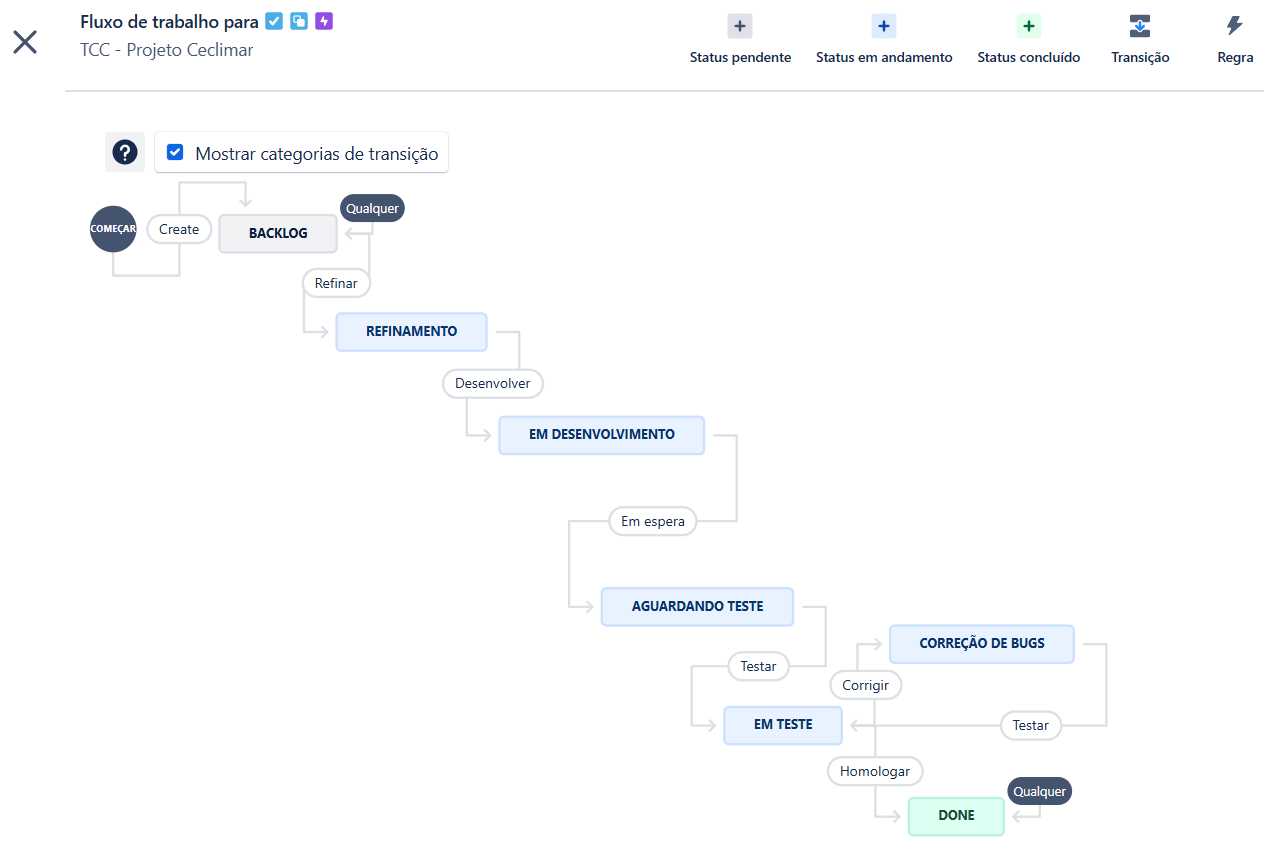
\includegraphics[width=0.8\textwidth]{imagens/fluxoJira.png}
    \caption{Fluxo de trabalho do Jira gerado para o desenvolvimento do projeto.}
    \legend{Fonte: Autor}
    \label{fig:fluxoJira}
\end{figure} 

O \textit{Backlog} é a coluna onde todas as tarefas, user stories e \textit{bugs} serão inicialmente posicionados. Nesta etapa, as tarefas serão priorizadas antes de andarem para o próximo estágio.

No Refinamento, as tarefas puxadas do \textit{Backlog} são detalhadas para um desenvolvimento mais assertivo. São refinados critérios de aceitação, estimativas de tempo e algum débito técnico.

As tarefas que estiverem em desenvolvimento são as que tiveram, efetivamente, o seu desenvolvimento iniciado. Assim que o desenvolvimento estiver finalizado, as tarefas serão transferidas para aguardando teste, onde ficarão até serem puxadas para testes mais detalhados.

No estágio de teste, os critérios de aceite e a presença de \textit{bugs} serão testados com o intuito de manter a qualidade do produto final. As tarefas que tiverem \textit{bugs} ou divergências de regras de negócio identificadas serão movidas para a coluna Correção de \textit{bugs} para que sejam corrigidas.

E, por último, após a homologação das tarefas nas etapas anteriores as tarefas são movidas para \textit{Done} que indicará sua finalização.

% ---

% ---
% Capitulo 3
% ---
\chapter{Cronograma}\label{cronograma}
% MARCELO 17/05: UNIR COM A SEÇÃO DO CAPÍTULO ANTERIOR.
O cronograma ilustrado na Tabela ~\ref{tab:cronograma} representa a trajetória de 
desenvolvimento do projeto ao longo de 16 meses, bem como as divergências e 
replanejamentos que foram realizados no decorrer do tempo. O trabalho teve seu 
início no dia 28 de março de 2024, com a realização de uma reunião de definição 
de escopo junto do orientador Marcelo Paravisi. No dia 1º de abril, deu-se 
continuidade com a definição do tema, em uma reunião externa com um membro do 
CECLIMAR. Essa etapa foi fundamental para delimitar o foco do trabalho e aprofundar 
a compreensão das dificuldades, necessidades, oportunidades e pontos críticos do projeto

Os meses seguintes, de maio a julho de 2024, foram dedicados à revisão bibliográfica 
e à definição metodológica. A definição metodológica se deu durante o mês de maio 
tendo início no dia 06, enquanto a parte de revisão bibliográfica se iniciou no 
dia 05 do mesmo mês e foi finalizada no final de julho. 

O levantamento de requisitos e regras de negócio se deu a partir do dia 10 de 
maio e se estendeu até o final de agosto para que os alinhamentos de definições 
com a equipe do CECLIMAR fossem mais abertos e constantes. É importante ressaltar 
que durante o desenvolvimento houve mudanças de funcionalidades e ajustes de regras 
de negócio durante o período de testes que fizeram com que fosse necessário 
revisitar esse tópico. 

Esse período inicial de estruturação se mostrou essencial para assegurar uma base 
sólida para iniciar o desenvolvimento. A parte de desenvolvimento técnica se 
iniciou com a organização da implementação do sistema no dia 20 de maio de 2024 
e, com base nisso, se iniciou a codificação do aplicativo no dia 1º de julho do mesmo ano. 

Inicialmente, o desenvolvimento tinha um planejamento de conclusão para o final 
de outubro, porém, embora as atividades tenham progredido conforme o cronograma, 
em uma reunião com o orientador do projeto foi decido realizar uma alteração no 
cronograma adicionando uma etapa de testes disponibilizando a aplicação com 
testadores tanto do projeto parceiro, como terceiros que contribuíram para que 
a aplicação adquirisse uma maturidade maior. Com isso, o prazo final de codificação 
foi replanejado para o início de maio de 2025 (Tabela ~\ref{tab:cronograma}).

A parte de redação da parte escrita do trabalho de conclusão foi iniciada 
no mês de junho para obter uma documentação mais precisa 
do processo e estava planejada para ser concluída até o final de novembro 
de 2024, porém, também foi afetada pelo replanejamento. Em vermelho na 
Tabela ~\ref{tab:cronograma} podemos ver que esta etapa foi realizada dentro 
do prazo previsto até o mes de outubro, porém em novembro foi adiada para maio 
e junho para priorizar a conclusão da codificação e o aprimoramento da qualidade 
da aplicação.
O desenvolvimento continuou sendo a atividade central até maio de 2025, acompanhado 
de execuções constantes de testes. No mês de maio de 2025 a redação do trabalho 
retornou e se estendeu, junto da revisão textual, até o final de junho para ser 
entregue dentro da data máxima de 26 de junho. A apresentação para a banca até o 
momento havia sido definida, porém tem prazo máximo de 11 de julho de 2025.

Esse cronograma evidencia o fluxo de trabalho realizado desde o início do 
planejamento do projeto, bem como as alterações ocorridas durante seu desenvolvimento. 
Para a elaboração desse material, foi fundamental que os períodos de escrita e codificação 
estivessem bem alinhados, permitindo traçar e documentar, com maior precisão, a linha do 
tempo apresentada, desde o início até a entrega final planejada.

% a tabela realmente ficou bem representativa? 
\begin{table}[ht]
\centering
\renewcommand{\arraystretch}{1.5}
\setlength{\tabcolsep}{4pt}
\resizebox{\textwidth}{!}{
\begin{tabular}{|>{\bfseries}l|*{11}{>{\centering\arraybackslash}p{1.6cm}|}}
\hline
\rowcolor{gray!20}
Meses & \rotatebox{90}{Reunião def. de escopo} & \rotatebox{90}{Definição de tema} & \rotatebox{90}{Revisão bibliográfica} & \rotatebox{90}{Def. metodológica} & \rotatebox{90}{Levantamento de requisitos  } & \rotatebox{90}{Organização de implementação} & \rotatebox{90}{Desenvolvimento} & \rotatebox{90}{Redação de TCC} & \rotatebox{90}{Revisão textual} & \rotatebox{90}{Apresentação} & \rotatebox{90}{Testes} \\ \hline
Mar/24 & \cellcolor{gray!30} & & & & & & & & & & \\ \hline
Abr/24 & & \cellcolor{gray!30} & & & & & & & & & \\ \hline
Mai/24 & & & \cellcolor{gray!30} & \cellcolor{gray!30} & \cellcolor{gray!30} & \cellcolor{gray!30} & & & & & \\ \hline
Jun/24 & & & \cellcolor{gray!30} & & \cellcolor{gray!30} & \cellcolor{gray!30} & & \cellcolor{gray!30} & & & \\ \hline
Jul/24 & & & \cellcolor{gray!30} & & \cellcolor{gray!30} & & \cellcolor{gray!30} & \cellcolor{gray!30} & & & \\ \hline
Ago/24 & & & & & \cellcolor{gray!30} & & \cellcolor{gray!30} & \cellcolor{gray!30} & & & \\ \hline
Set/24 & & & & & & & \cellcolor{gray!30} & \cellcolor{gray!30} & & & \\ \hline
Out/24 & & & & & & & \cellcolor{gray!30} & \cellcolor{gray!30} & & & \\ \hline
Nov/24 & & & & & & & \cellcolor{blue!30} & \cellcolor{red!30} & \cellcolor{red!30} & & \\ \hline
Dez/24 & & & & & & & \cellcolor{blue!30} & & & \cellcolor{red!30} & \cellcolor{blue!30} \\ \hline
Jan/25 & & & & & & & \cellcolor{blue!30} & & & & \cellcolor{blue!30} \\ \hline
Fev/25 & & & & & & & \cellcolor{blue!30} & & & & \cellcolor{blue!30} \\ \hline
Mar/25 & & & & & & & \cellcolor{blue!30} & & & & \cellcolor{blue!30} \\ \hline
Abr/25 & & & & & & & \cellcolor{blue!30} & & & & \cellcolor{blue!30} \\ \hline
Mai/25 & & & & & & & \cellcolor{blue!30} & \cellcolor{blue!30} & & & \cellcolor{blue!30} \\ \hline
Jun/25 & & & & & & & & \cellcolor{blue!30} & \cellcolor{blue!30} & \cellcolor{blue!30} & \cellcolor{blue!30} \\ \hline
\end{tabular}%
}
\caption{Cronograma de desenvolvimento — Cinza: Planejamento inicial, Azul: Replanejamento, Vermelho: Prazos adiados.}
\label{tab:cronograma}
\legend{Fonte: Autor}
\end{table}
% ---

% Capitulo 4
% ---

\chapter{Referencial Teórico}\label{referencial-teorico}

% ---
\section{Ciência Cidadã}
% ---

A Ciência Cidadã representa uma ponte entre a comunidade científica e o público geral, permitindo que pessoas sem formação científica formal possam contribuir em pesquisas científicas. Essa metodologia colaborativa tem se destacado em diversas áreas de pesquisa como na conservação da biodiversidade e na preservação ambiental. Através da Ciência Cidadã é possível que voluntários coletem e analisem dados, fornecendo informações que agregam no conhecimento acadêmico e auxiliam na resolução de questões sociais.

Segundo \citeonline{palma2016monitoramento}, trata-se de uma metodologia de pesquisa promissora na produção de conhecimento para ser aplicada em diversos campos científicos. Essa abordagem se destaca, em especial, com seu potencial de  geração de dados e análises, temporal e espacial, quando comparada com os métodos tradicionais de pesquisa. Para \citeonline{wildschut2017citizen}, a metodologia da ciência cidadã tem potencial para ampliar o escopo de pesquisas e aumentar e aprimorar a capacidade na coleta de dados e que os cidadãos que participam podem contribuir com informações importantes enquanto aprendem sobre as mais diversas áreas científicas.

A construção de conhecimento colaborativo realizado entre cidadãos e cientistas se mostra uma maneira poderosa de construção de conhecimentos, que agrega tanto no meio científico quanto social. Estes projetos instigam que as pessoas participem de maneira voluntária e ativa na resolução de situações do dia-a-dia da nossa sociedade, disseminando conhecimento de diversas áreas e fazendo com que diversos conteúdos saiam de suas bolhas científicas e obtenham um alcance maior.

% ---
\section{Agenda 2030}
% ---

A Agenda 2030 para o Desenvolvimento Sustentável é um plano de ação global adotado pelas Nações Unidas em 2015, com o objetivo de promover a prosperidade enquanto protege o planeta. Ela estabelece 17 Objetivos de Desenvolvimento Sustentável (ODS), que são subdivididos em 169 metas específicas. Esses objetivos englobam uma ampla gama de questões sociais, econômicas e ambientais, como erradicação da pobreza, igualdade de gênero, educação de qualidade, água limpa e saneamento, energia acessível e não poluente, trabalho decente e crescimento econômico \cite{onu2015ods}.

Segundo a organização, os ODS são projetados com os três pilares do desenvolvimento sustentável: econômico, social e ambiental. A Agenda enfatiza a importância de garantir que os direitos humanos de todos sejam realizados e que haja igualdade de gênero e empoderamento de mulheres e meninas. Além disso, reconhece que a erradicação da pobreza em todas as suas formas é o maior desafio global e, um requisito indispensável para o desenvolvimento sustentável.

A implementação da Agenda 2030 requer a mobilização de recursos e uma Parceria Global para o Desenvolvimento Sustentável, envolvendo todos os países, partes interessadas e pessoas. A Agenda é mundial, e se aplica a todos os países levando em conta diferentes realidades nacionais, capacidades e níveis de desenvolvimento. Ela promove a paz, justiça e instituições eficazes, e destaca a necessidade de ações urgentes sobre a mudança climática para proteger o planeta para as gerações presentes e futuras \cite{onu2015agenda2030}.

% ---
\section{Objetivos de Desenvolvimento Sustentável (ODS)}
% ---

Os ODS são um conjunto de 17 metas estabelecidas pelas Nações Unidas para abordar os principais desafios de desenvolvimento no Brasil e em todo o mundo. Esses objetivos visam criar um futuro mais justo, equitativo e sustentável para todos \cite{onu2015ods}. São eles:

\begin{enumerate}
    \item \textbf{ODS 1}: Erradicação da Pobreza: Acabar com a pobreza em todas as suas formas, em todos os lugares.
    \item \textbf{ODS 2}: Fome Zero e Agricultura Sustentável: Garantir a segurança alimentar, melhorar a nutrição e promover a agricultura sustentável.
    \item \textbf{ODS 3}: Saúde e Bem-Estar: Assegurar uma vida saudável e promover o bem-estar para todas as idades.
    \item \textbf{ODS 4}: Educação de Qualidade: Garantir uma educação inclusiva, equitativa e de qualidade.
    \item \textbf{ODS 5}: Igualdade de Gênero: Alcançar a igualdade de gênero e empoderar todas as mulheres e meninas.
    \item \textbf{ODS 6}: Água Limpa e Saneamento: Garantir a disponibilidade e gestão sustentável da água e saneamento para todos.
    \item \textbf{ODS 7}: Energia Limpa e Acessível: Assegurar o acesso a fontes de energia acessíveis, confiáveis, sustentáveis e modernas.
    \item \textbf{ODS 8}: Trabalho Decente e Crescimento Econômico: Promover o crescimento econômico inclusivo e sustentável, emprego pleno e produtivo e trabalho decente para todos.
    \item \textbf{ODS 9}: Indústria, Inovação e Infraestrutura: Construir infraestruturas resilientes, promover a industrialização inclusiva e sustentável e fomentar a inovação.
    \item \textbf{ODS 10}: Redução das Desigualdades: Reduzir as desigualdades dentro e entre países.
    \item \textbf{ODS 11}: Cidades e Comunidades Sustentáveis: Tornar as cidades e os assentamentos humanos inclusivos, seguros, resilientes e sustentáveis.
    \item \textbf{ODS 12}: Consumo e Produção Responsáveis: Assegurar padrões de consumo e produção sustentáveis.
    \item \textbf{ODS 13}: Ação Contra a Mudança Global do Clima: Tomar medidas urgentes para combater a mudança climática e seus impactos.
    \item \textbf{ODS 14}: Vida na Água: Conservar e usar de forma sustentável os oceanos, mares e recursos marinhos.
    \item \textbf{ODS 15}: Vida Terrestre: Proteger, restaurar e promover o uso sustentável dos ecossistemas terrestres, gerir florestas de forma sustentável, combater a desertificação e deter a perda de biodiversidade.
    \item \textbf{ODS 16}: Paz, Justiça e Instituições Eficazes: Promover sociedades pacíficas e inclusivas para o desenvolvimento sustentável, proporcionar acesso à justiça para todos e construir instituições eficazes, responsáveis e inclusivas em todos os níveis.
    \item \textbf{ODS 17}: Parcerias e Meios de Implementação: Fortalecer os meios de implementação e revitalizar a parceria global para o desenvolvimento sustentável.
\end{enumerate}

Os itens acima são um apelo global visando acabar com a pobreza, proteger o meio ambiente e o clima e garantir que as pessoas, em todos os lugares, possam desfrutar de paz e de prosperidade. São objetivos nos quais as Nações Unidas estão contribuindo para atingir a Agenda 2030 no Brasil \cite{onu2015ods}.

% ---
\section{Metodologia Iterativa Incremental}
% ---
A metodologia iterativa incremental é uma abordagem de desenvolvimento de \textit{software} que divide o processo em ciclos repetitivos. Cada iteração resulta em uma versão incrementada do \textit{software}, que é construída sobre a versão anterior com adições e melhorias. Segundo \citeonline{pressman2011engenharia}, essa metodologia permite que as equipes avaliem e integrem feedbacks mais rapidamente, adaptando-se às mudanças e refinando o produto ao longo do tempo. Isso contrasta com o modelo tradicional em cascata, onde cada fase deve ser concluída antes da próxima começar, sem retorno para fases anteriores.

De acordo com \citeonline{pressman2011engenharia}, o modelo incremental é uma abordagem de desenvolvimento de \textit{software} que foca na entrega gradual de funcionalidades em sucessivas versões incrementais. Nesse modelo, o desenvolvimento do \textit{software} é dividido em várias partes ou incrementos, cada um entregando uma versão operante do produto, que é aprimorada e expandida em lançamentos subsequentes.

\citeonline{pressman2011engenharia} afirma que o modelo incremental integra elementos de fluxos de processos lineares e paralelos. Na Figura~\ref{fig:incremental} é possível observar essa relação a partir das sequências lineares de forma escalonada que demonstram que ao longo do tempo cada incremento adiciona funcionalidades ou aprimoramentos ao sistema, permitindo uma evolução constante e contínua do produto final.

\begin{figure}[htb]
  \centering
  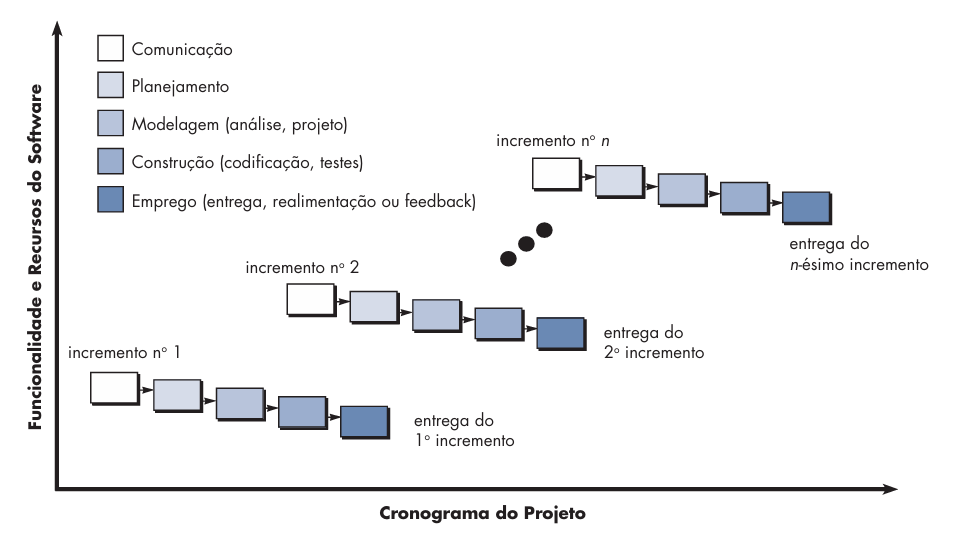
\includegraphics[width=0.8\textwidth]{imagens/graficoPressman.png}
  \caption{Ciclo de desenvolvimento incremental.}
  \legend{Fonte: \citeonline{pressman2011engenharia}.}
  \label{fig:incremental}
\end{figure}

% ---
\section{Kanban}
% ---

O Kanban é um método de gestão de fluxo de trabalho que fornece uma visualização das tarefas que devem ser realizadas, quando entregá-las e quanto ainda é necessário para finalizá-las com o objetivo de aumentar a eficiência e o entendimento do desenvolvimento \cite{ohno1988toyota}. Originou-se no sistema da Toyota no Japão dos anos 1940 e foi adaptado para o desenvolvimento de \textit{software} e sistemas de TI por David J. Anderson em 2004. Para isso, o Kanban utiliza de um quadro dividido em colunas para representar os diferentes estágios do trabalho, onde os cartões que representam as tarefas se movem de uma coluna para outra, refletindo o progresso real \cite{zayat2020framework}.

% ---
\section{Jira}
% ---

O Jira é um \textit{software} comercial de gerenciamento de projetos desenvolvido pela empresa Atlassian. Ele permite a criação, acompanhamento e gerência de tarefas e projetos a partir de uma interface personalizável que suporta diversas metodologias ágeis como Scrum e Kanban, facilitando a colaboração e comunicação durante o desenvolvimento.

A ferramenta pode ser usada para planejar \textit{sprints}, atribuir tarefas, acompanhar \textit{bugs}, gerar relatórios e analisar o desempenho da equipe. Ele possui integração com uma variedade de ferramentas de desenvolvimento e oferece funcionalidades para personalizar fluxos de trabalho, campos e painéis, tornando-o adaptável às necessidades específicas de cada projeto ou organização.

% ---

% Capitulo 5
% ---
\chapter{Trabalhos Correlatos}\label{trabalhos-correlatos}

Com o intuito de contextualizar e ter uma melhor visão de onde posicionar o projeto dentro do campo de pesquisa escolhido, foi realizada uma seleção de trabalhos correlatos, cujos principais critérios de aceitação incluíram a abordagem de temas como: monitoramento de fauna, desenvolvimento sustentável, gestão ambiental e ciência cidadã. Garantindo assim, relevância e alinhamento do projeto com as necessidades e avanços da área.

O ponto de partida para as pesquisas foi o \citeonline{sibbr2024}. A plataforma online, pertencente ao sistema gov.br \cite{govbr2024}, que integra dados e informações sobre a biodiversidade e os ecossistemas de diversas fontes, os tornando acessíveis e livres para usos diversos. Nele, também é possível ter acesso ao sistema Ciência Cidadã, que consiste em uma colaboração entre a comunidade e cientistas na coleta de dados para pesquisa científica. 

A partir do levantamento bibliográfico, pesquisas na plataforma Play Store \cite{playstore2024}, presente nos dispositivos Android \cite{android2024}, foram realizadas baseadas em alguns projetos e palavras-chave pré-selecionadas. As principais palavras-chave usadas para realizar as buscas foram: animais costeiros, coleta de dados, monitoramento ambiental, ciência cidadã.

Nesta seção, serão apresentadas três aplicações separadas no levantamento documental que  demonstraram possuir características e funcionalidades que podem auxiliar na definição e desenvolvimento deste sistema. Estas aplicações possuem algumas características em comum, porém cada uma delas também traz características únicas que serão importantes balizadoras nas tomadas de decisão deste projeto.

% ---
\section{SISS-Geo}\label{siss-geo}
% --- 

O Sistema de Informação em Saúde Silvestre (SISS-Geo) da FIOCRUZ é desenvolvido pela Plataforma Institucional Biodiversidade e Saúde Silvestre, com apoio do Laboratório Nacional de Computação Científica. É gratuito, disponível em \textit{smartphones} e na \textit{web}, para o monitoramento da saúde dos animais silvestres em ambientes naturais, rurais e urbanos. Apoia a investigação da ocorrência de agentes causadores de doenças, como agentes infecciosos, que podem acometer pessoas e animais. Como instrumento de ciência cidadã torna possível, a partir de registros realizados por cidadãos comuns, profissionais de saúde, meio ambiente, pesquisadores e especialistas em vida silvestre, agir para a prevenção e controle de zoonoses e a conservação da biodiversidade brasileira \cite{chame2015sissgeo}.

\begin{figure}[htb]
  \centering
  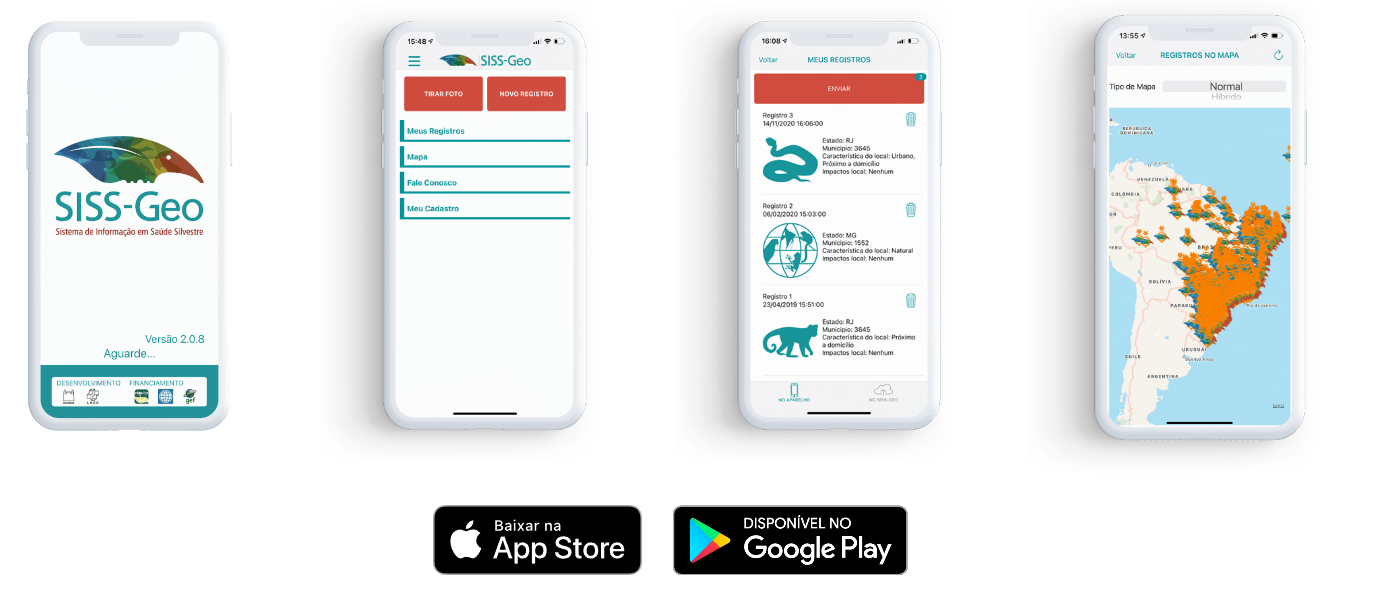
\includegraphics[width=1\textwidth]{imagens/sisGeoApp.png}
  \caption{Interface do sistema SISS-Geo.}
  \legend{Fonte: \citeonline{plataforma2024sissgeo}.}
  \label{fig:sisgeoApp}
\end{figure}

A aplicação \textit{mobile} foi lançada em 2014 e está disponível tanto para IOS quanto para Android (Figura~\ref{fig:sisgeoApp}) e possui mais de 10.000 downloads, com avaliação média de 4,7/5 baseada em 116 avaliações de usuários. Foram registrados, até 26 de março de 2024, 33 mil registros e quase 13 mil usuários colaboradores.

O sistema é bem consolidado e amplamente utilizado no Brasil, possuindo uma ótima aceitação entre especialistas e cidadãos em diversas regiões do país. Apesar de possuir opções para identificação de dados da fauna costeira, estes se mostram limitados quando comparados com os demais biomas. Ao alterar a escala de análise, é possível perceber, com um recorte mais detalhado do cordão litorâneo, que este não é o principal foco da aplicação e, atualmente, ela possui uma participação muito maior nas regiões continentais (Figura~\ref{fig:sisgeoMap}).

\begin{figure}[htb]
  \centering
  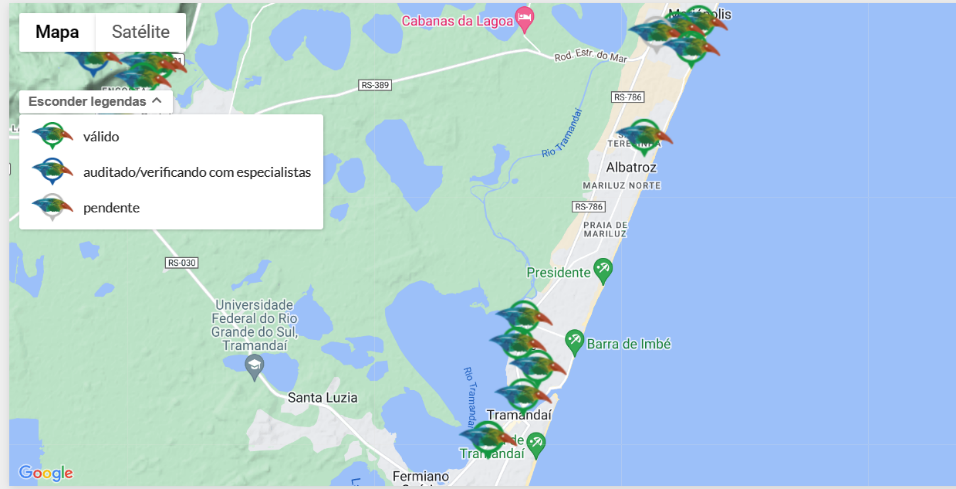
\includegraphics[width=1\textwidth]{imagens/sisGeoMapa.png}
  \caption{Recorte da região costeira do litoral norte do Rio Grande do Sul.}
  \legend{Fonte: \citeonline{plataforma2024sissgeo}.}
  \label{fig:sisgeoMap}
\end{figure}

Principais pontos fortes: funcionalidade \textit{offline}, iniciativa ambiental de grande contribuição, aplicação leve, ideia colaborativa de preservação, georreferenciamento de dados com boa visualização.

Entre as principais reclamações dos usuários estão: sistema pouco intuitivo, poucas opções de animais pré-cadastrados, interface confusa com formulário por vezes muito técnico.

% ---
\section{Sistema Urubu}\label{urubu}
% --- 

O Sistema Urubu é uma iniciativa do Centro Brasileiro de Ecologia de Estradas da UFLA, sob a coordenação do professor Alex Bager. Criado em 2014, o aplicativo de ciência cidadã é a maior rede para conservação da biodiversidade brasileira, destinada à coleta e gestão de informações de fauna selvagem ao longo de rodovias e ferrovias no Brasil. 

A aplicação permite que voluntários enviem registros de animais atropelados e infraestruturas viárias por meio de aplicativo móvel, enquanto especialistas validam e caracterizam esses registros para torná-los confiáveis. Os dados coletados são centralizados em um banco de dados e disponibilizados em um Sistema de Informações Geográficas, facilitando a visualização e análise pelos usuários. O Sistema Urubu também oferece ferramentas como o Urubu \textit{web}, para gestão e validação dos dados, e o Urubu Map, para visualização geográfica dos registros \cite{castro2019sistema}. Ao longo de seus anos de existência, o sistema reuniu mais de 25 mil usuários e 150 mil registros de animais atropelados em todo o território brasileiro, demonstrando seu impacto e relevância na conservação da biodiversidade.

\begin{figure}[htb]
  \centering
  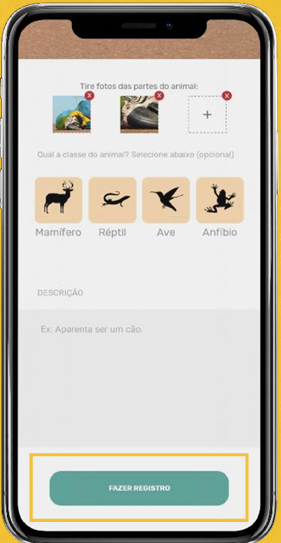
\includegraphics[width=0.33\textwidth]{imagens/app1.png}
  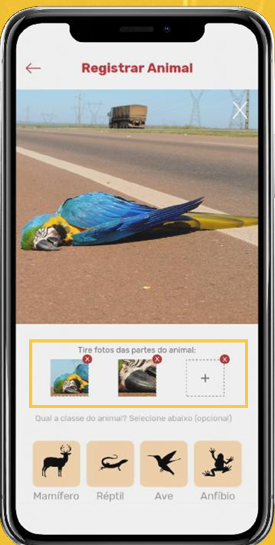
\includegraphics[width=0.323\textwidth]{imagens/app3.png}
  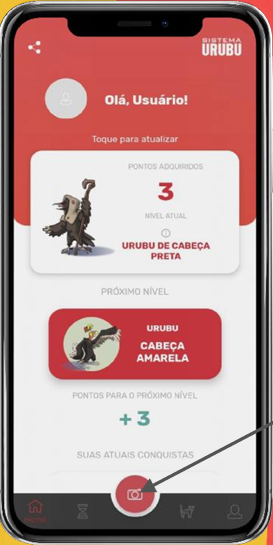
\includegraphics[width=0.32\textwidth]{imagens/app2.png}
  \caption{Interface do Sistema Urubu.}
  \legend{Fonte: Capturas de tela do sistema urubu disponíveis no manual de uso do aplicativo.}
  \label{fig:urubuApp}
\end{figure}

O Sistema Urubu apresenta uma interface amigável e um fluxo de obtenção e envio de dados de registros intuitivo (Figura~\ref{fig:urubuApp}.a e ~\ref{fig:urubuApp}.b), além de um fluxo gamificado com progressão recompensada para os usuários que contribuem com o projeto (Figura~\ref{fig:urubuApp}.c).

O fluxo de funcionamento da aplicação se inicia com a morte de algum animal em uma rodovia ou ferrovia, quando esse animal é encontrado por usuário a entrada de registro pode ser realizada via \textit{mobile}, \textit{web} ou por importação via planilha de Excel. Os dados de cada registro são então passados por uma análise de profissionais que decidirão se serão inseridos nos dados finais.

Apesar de ter alcançado importantes números de aceitação e uso entre 2014 e 2023, atualmente o sistema se encontra desativado e indisponível para download em todas as plataformas e seu site se encontra fora do ar.

Em contato com o coordenador do projeto Alex Brag por e-mail, foi informado de que o Sistema Urubu foi desativado devido a falta de recursos. Segundo seu relato, além dos custos para manter a aplicação no ar com investimentos contínuos, os aplicativos de ciência cidadã requerem muita comunicação e relacionamento com os participantes, o que torna a estrutura mais complexa e custosa.

% ---
\section{SIMBA}\label{simba}
% --- 

O Sistema de Monitoramento da Biota Aquática (SIMBA), é um sistema \textit{web} de gerenciamento de dados criado pelo Laboratório de Oceanografia Biológica da UNIVALI com a finalidade de armazenar dados coletados por instituições executoras dos projetos de monitoramentos de praias. O desenvolvimento do SIMBA se iniciou para auxiliar nos fluxos de dados entre os atores sociais envolvidos nos Projetos de Monitoramento de Praias (PMPs) e fazer com que os dados obtidos sejam disponibilizados e divulgados para a população.

Os PMPs são desenvolvidos para o atendimento de condicionantes de licenciamento ambiental federal, conduzido pelo IBAMA, de atividades de exploração e produção de petróleo e gás natural de bacias \textit{offshore} sob atuação da Petrobras. Estes projetos tem o objetivo de avaliar as possíveis interferências na área de abrangência dos projetos, analisando tanto tetrápodes marinhos (aves, tartarugas e mamíferos) por meio do monitoramento das praias, atendimento veterinário aos animais debilitados e da coleta de dados de animais mortos, quanto resíduos sólidos encontrados \cite{petrobras_simba_2024}.

Atualmente os projetos estão presentes nas bacias de Santos, Campos, Espírito Santo, Sergipe-Alagoas e Potiguar.

\begin{figure}[htb]
  \centering
  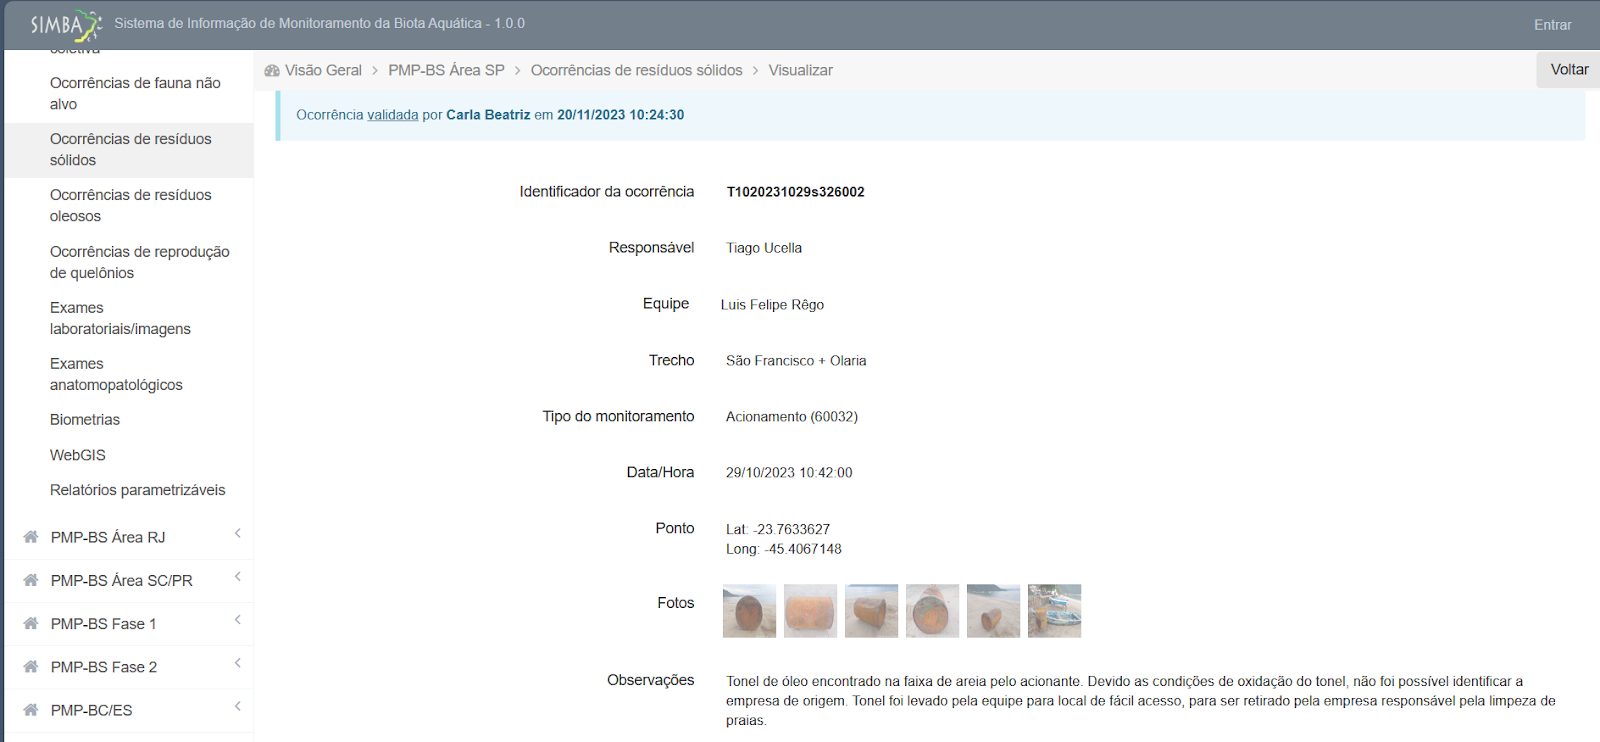
\includegraphics[width=1\textwidth]{imagens/simbaRegistro.png}
  \caption{Captura de tela de uma página \textit{web} de registro de visualização de ocorrências cadastradas no SIMBA.}
  \legend{Fonte: \cite{petrobras_simba_2024}.}
  \label{fig:simbaRegistro}
\end{figure}

O SIMBA conta com funcionalidades de cadastro de ocorrências de fauna, resíduos sólidos (Figura~\ref{fig:simbaRegistro}), exames, jornadas de campo com os caminhamentos realizados. Os pontos de ocorrência de cada cadastro são georreferenciados, assim como as jornadas de monitoramento, gerando mapas para melhor visualização e análise dos dados (Figura~\ref{fig:simbaMonitoramento}).

\begin{figure}[htb]
  \centering
  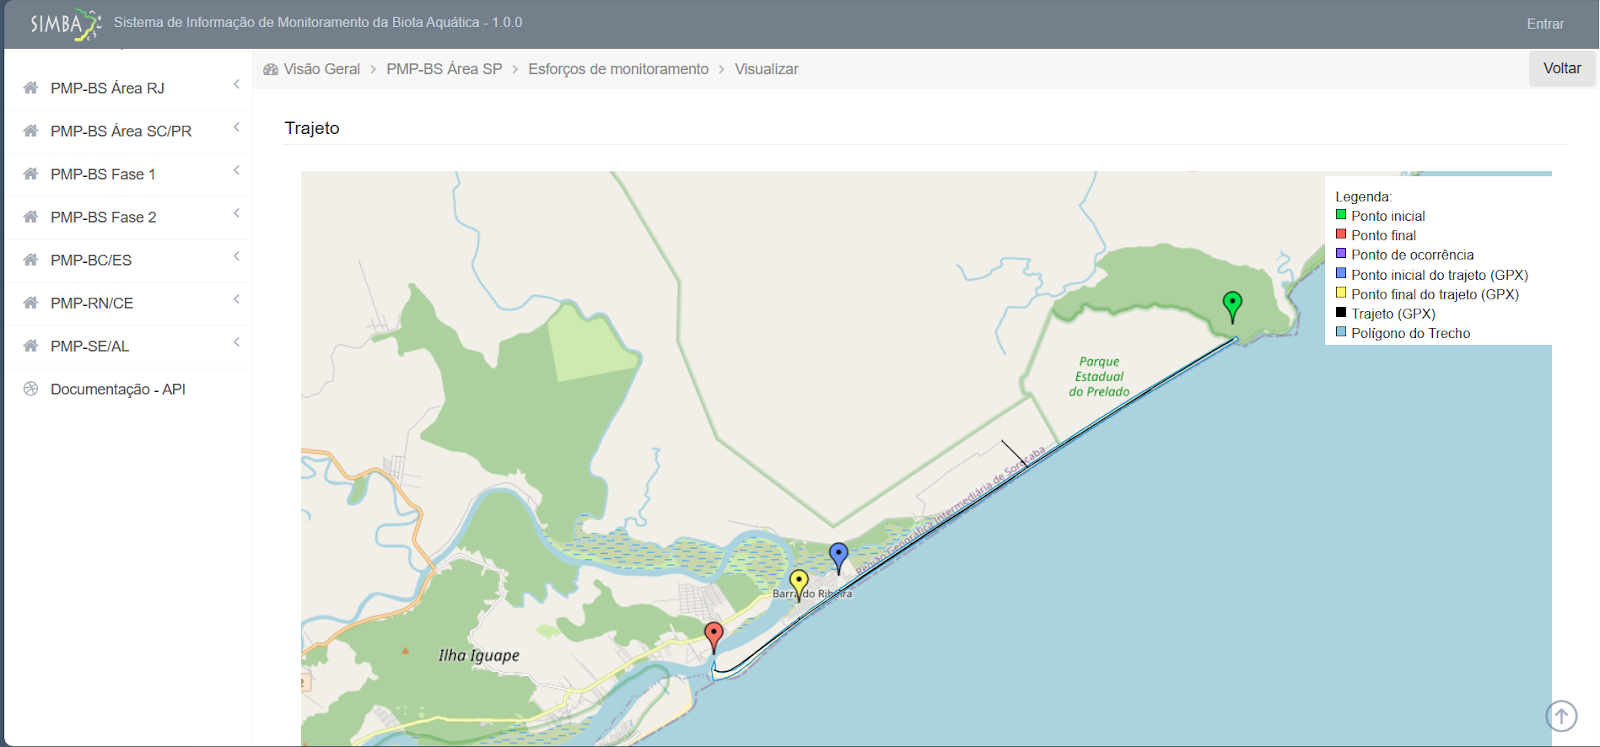
\includegraphics[width=1\textwidth]{imagens/simbaTrajetoria.png}
  \caption{Captura de tela de um mapa georreferenciado gerado a partir dos dados de jornada de monitoramento cadastrado no SIMBA.}
  \legend{Fonte: \cite{petrobras_simba_2024}.}
  \label{fig:simbaMonitoramento}
\end{figure}

O sistema possui uma área de acesso liberada ao público onde é possível visualizar dados já levantados e validados e uma área de acesso restrito liberada para pesquisadores. Possui uma interface mais limpa e direta, atendendo a um estilo de aplicação profissional apenas com o conteúdo necessário (Figura~\ref{fig:simbaPaginaCadastro}). Os dados são bem organizados e acessíveis para quem estiver interessado em acompanhar os estudos e evidências coletadas. Porém, para leigos essa interface pode, inicialmente, trazer um pouco de estranheza devido ao visual menos apelativo e aos termos mais científicos apresentados.

\begin{figure}[htb]
  \centering
  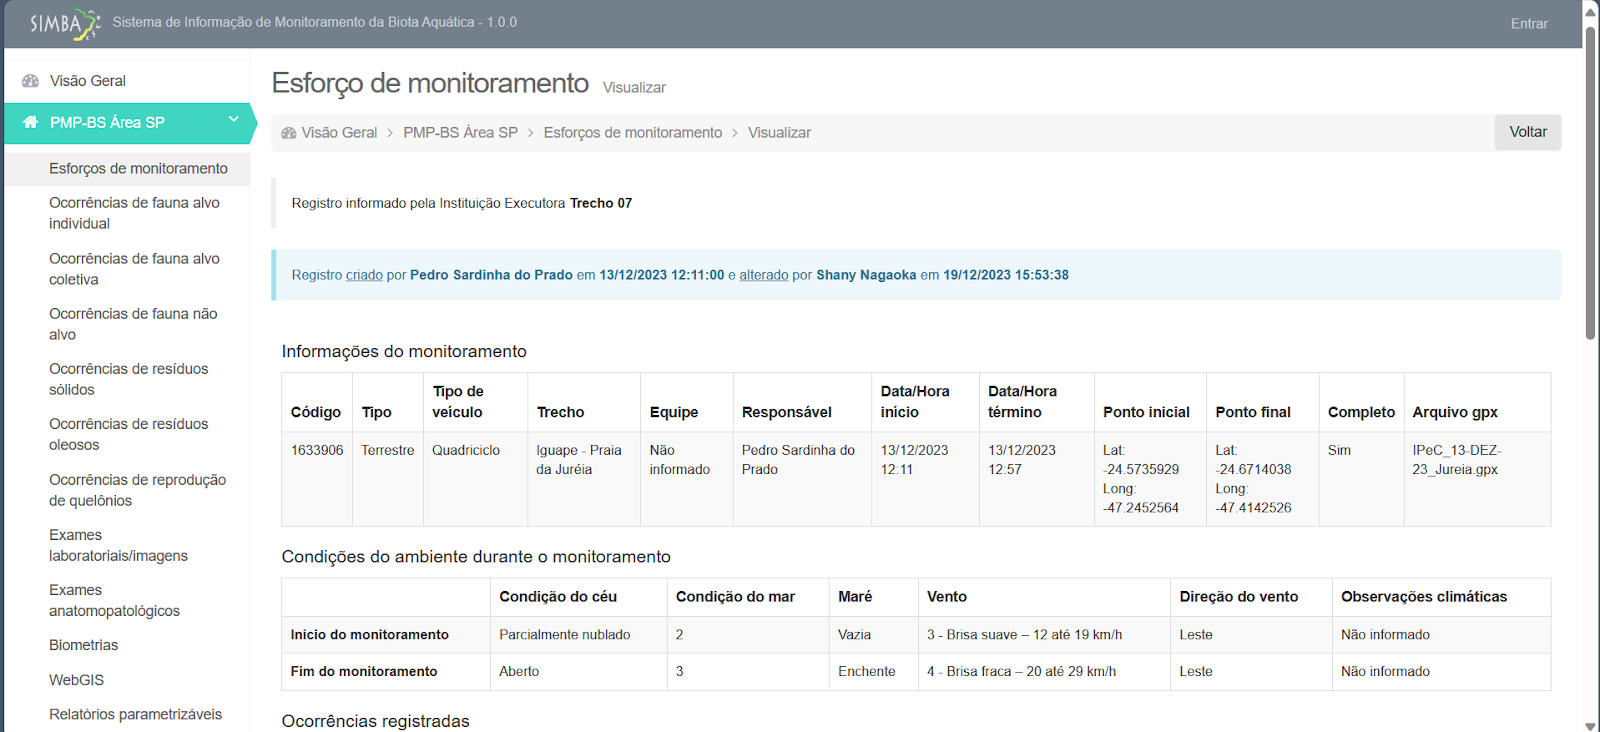
\includegraphics[width=1\textwidth]{imagens/simbaMonitoramento.png}
  \caption{Captura de tela da página \textit{web} de monitoramento cadastrada no SIMBA.}
  \legend{Fonte: \cite{petrobras_simba_2024}.}
  \label{fig:simbaPaginaCadastro}
\end{figure}

A geração de mapas georreferenciados e a possibilidade de uso \textit{offline} são aspectos importantes a serem destacados, pois permitem uma melhor análise e acompanhamento gráfico dos dados coletados e possibilitam que estes dados sejam obtidos até mesmo em locais mais isolados sem conexão com a internet. Outra função interessante é a liberação de dados para o público geral que se mostrar interessado em acompanhar os resultados e andamentos dos estudos nas praias onde os PMPs estão sendo realizados.

\section{Análise Comparativa e Direcionamentos do Projeto}

Com a análise dos principais trabalhos correlatos existentes, foi possível levantar os principais pontos de sucesso e alguns aspectos que precisam de melhorias, os quais influenciam diretamente na capacidade de sistemas similares alcançarem seus objetivos e obterem a aceitação do público-alvo.

A receptividade do Sistema Urubu e do SISS-Geo indicou um interesse significativo da população em participar de projetos de ciência cidadã, evidenciado pelos números expressivos de \textit{downloads} e registros de dados apresentados anteriormente.

Cada um dos três sistemas possui suas peculiaridades e objetivos distintos: enquanto o SISS-Geo está mais voltado ao monitoramento da saúde de animais silvestres e à investigação de agentes causadores de doenças, o Sistema Urubu foca principalmente no monitoramento de animais atropelados em rodovias e ferrovias. Por sua vez, o SIMBA busca fornecer visibilidade ao monitoramento costeiro realizado em regiões de exploração e produção de petróleo.

Sendo assim, a partir da análise prévia, foi possível constatar que existe uma oportunidade de posicionamento para o sistema proposto neste projeto, que se enquadra como uma plataforma com interface amigável e intuitiva, visando otimizar o processo de coleta, classificação e gestão de dados da fauna costeira. O sistema poderá se apoiar em pontos fortes identificados nos sistemas correlatos, como a funcionalidade offline do SISS-Geo, a interface amigável do Sistema Urubu e a organização dos dados do SIMBA.

O sistema proposto buscará oferecer uma experiência de usuário agradável e descomplicada para o registro de observações da fauna costeira, com opções abrangentes de espécies para classificação e ferramentas de visualização de dados claras e acessíveis. Ao adotar uma abordagem centrada no usuário e priorizar a simplicidade e eficiência, pretende-se ampliar o engajamento da comunidade na coleta de dados científicos e contribuir significativamente para o monitoramento e conservação da biodiversidade costeira.

% ---

% ---
% Conclusão
% ---
\chapter{Conclusão}
% ---

\lipsum[31-33]
% ---


% ----------------------------------------------------------
% ELEMENTOS PÓS-TEXTUAIS
% ----------------------------------------------------------
\postextual
% ----------------------------------------------------------

% ----------------------------------------------------------
% Referências bibliográficas (Obrigatório)
% ----------------------------------------------------------
\bibliography{elementos-pos-textuais/referencias}


% ----------------------------------------------------------
% Glossário (Opcional)
% ----------------------------------------------------------
%
% Consulte o manual da classe abntex2 para orientações sobre o glossário.
%
%\glossary


% ----------------------------------------------------------
% Apêndices (Opcional)
% ----------------------------------------------------------
% ---
% Inicia os apêndices
% ---
\begin{apendicesenv}

% ----------------------------------------------------------
\chapter{Quisque libero justo}
% ----------------------------------------------------------

\lipsum[50]
% ----------------------------------------------------------
\chapter{Nullam elementum urna vel imperdiet sodales elit ipsum pharetra ligula
ac pretium ante justo a nulla curabitur tristique arcu eu metus}
% ----------------------------------------------------------
\lipsum[55-57]

\end{apendicesenv}
% ---


% ----------------------------------------------------------
% Anexos (Opcional)
% ----------------------------------------------------------
% ---
% Inicia os anexos
% ---
\begin{anexosenv}

% ---
\chapter{Morbi ultrices rutrum lorem.}
% ---
\lipsum[30]
% ---
\chapter{Cras non urna sed feugiat cum sociis natoque penatibus et magnis dis
parturient montes nascetur ridiculus mus}
% ---

\lipsum[31]
% ---
\chapter{Fusce facilisis lacinia dui}
% ---

\lipsum[32]

\end{anexosenv}


%---------------------------------------------------------------------
% INDICE REMISSIVO (Opcional)
%---------------------------------------------------------------------
%\phantompart
%\printindex
%---------------------------------------------------------------------

\end{document}
